\chapter{Súvisiace práce}

\label{kap:suvisiace_prace} % id kapitoly pre prikaz ref

TODO

\section{Prieskumník štruktúr}
\label{sec:explorer}

Prieskumník štruktúr je jednou z webových aplikácií používaných na predmete Logika pre informatikov. Jej úlohou je poskytnúť študentom interaktívny pohľad na štruktúry pre jazyky logiky prvého rádu. Primárne umožňuje definovanie vlastného jazyka a štruktúry logiky prvého rádu, v rámci ktorej možno následne skúmať pravdivosť formúl.

Pôvodná aplikácia vznikla v rámci viacerých bakalárskych prác. Konkrétne sa jedná o prácu Milana Cifru \cite{cifra2018}, ktorá sa zaoberá samotným vývojom prieskumníka štruktúr, prácu Richarda Tótha \cite{toth2021}, rozširujúcu prieskumník o Henkinovu-Hintikkovu hru a prácu Miroslava Baluchu \cite{baluch2020}, ktorá priniesla alternatívny grafový pohľad. Túto poslednú prácu ešte bližšie rozoberieme v nasledujúcej podkapitole \ref{sec:graph-explorer}.

Implementácia aplikácia sa však časom stala neaktuálnou a nejednotnou, keďže bola výsledkom viacerých bakalárskych prác využívajúcich rôzne prístupy k použitým technológiám. To spôsobilo jej ťažkú udržateľnosť, ako aj náročnosť rozširovania o ďalšiu funkcionalitu.

Cieľom bakalárskej práce Jozefa Filipa \cite{filip2025} bolo vytvorenie novej, jednotnej verzie pôvodnej aplikácie bez grafového pohľadu a novým spôsobom využitia Henkinovej-Hintikkovej hry. Túto verziu možno vidieť na obrázku \ref{obr:old_se}.

\begin{figure}
    \centerline{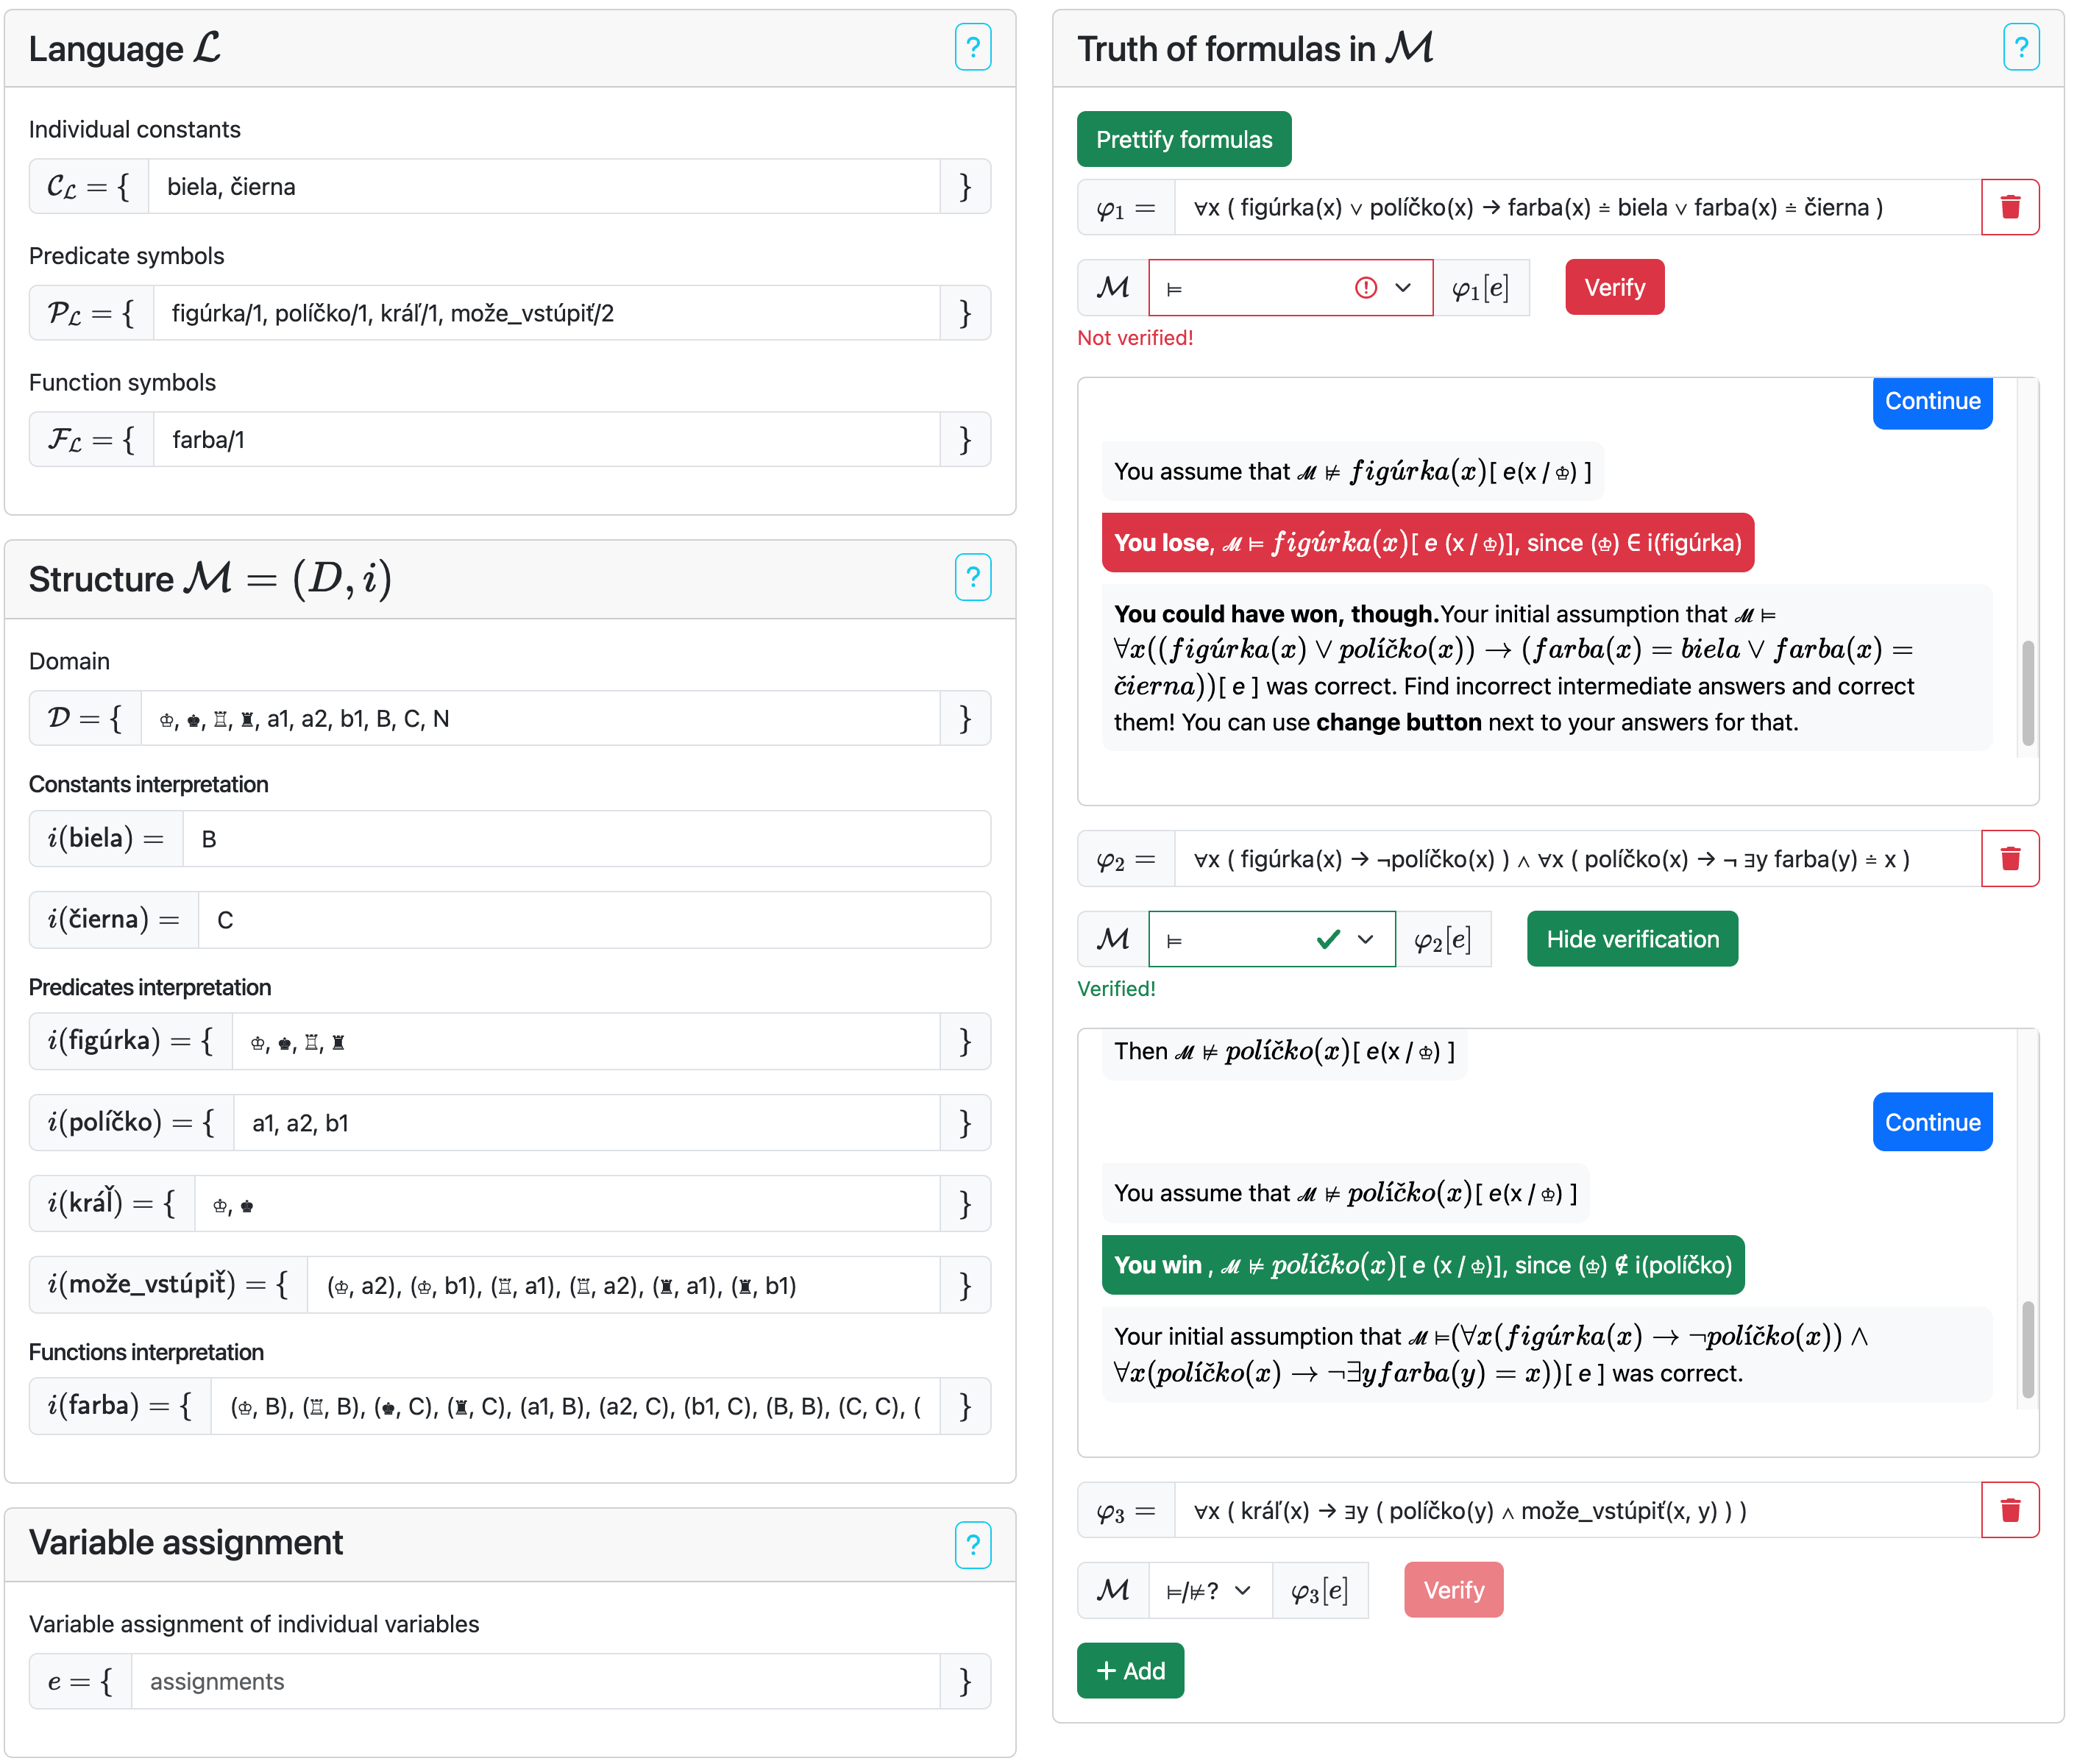
\includegraphics[width=1\textwidth]{images/old_se2.png}}
    %popis obrazku
    \caption[Používateľské rozhranie reimplentovanej verzie Prieskumníka štruktúr.]{Používateľské rozhranie reimplentovanej verzie Prieskumníka štruktúr.}
    %id obrazku, pomocou ktoreho sa budeme na obrazok odvolavat
    \label{obr:old_se}
\end{figure}


V ľavej hornej časti obrázka sa nachádzajú textové vstupy na definovanie mimologický symbolov. V prípade predikátových a funkčných symbolov sa definuje aj ich arita vo formáte \textit{symbol/arita}. Pod definíciou jazyka logiky prvého rádu sa definuje samotná štruktúra, to vyžaduje zadanie domény a určenie interpretácie jednotlivých mimologických symbolov. Aplikácia poskytuje iba jeden, tzv. množinový pohľad na interpretáciu predikátových a funkčných symbolov, ktorý je opäť realizovaný pomocou textového vstupu.

V pravej časti aplikácie používateľ definuje formuly. Po vytvorení validného jazyka a štruktúry môže skúmať splniteľnosť týchto formúl v danej štruktúre. Na zistenie splniteľnosti musí používateľ najprv zadať svoj tip, či je formula splniteľná, alebo nie. Na overenie svojho tipu si musí zahrať Henkinovu-Hintikkovu hru, po ktorej skončení zistí dôvod správnosti alebo nesprávnosti svojho pôvodného tipu.

\section{Prieskumník grafových štruktúr}
\label{sec:graph-explorer}

TODO

\section{Logický pracovný zošit}
\label{sec:workbook}

TODO